\chapter{システムの実装方法}
\label{chp:reference}

\section{システム構成}
\label{sec:reference_ftnote}
本システムは以下のような構成で実装を行う.システム構成図を図3.1に示す.\\
労務管理支援システムをReactでWebアプリとして作成した.さらにデータベースにCloud Firestore,
ユーザー認証にFirebase Authentication,表情分析にface-api.jsを使用した。\\
 次のセクションでは,それぞれのサービスについて説明する.

\begin{figure}[!h]
	\begin{center}
			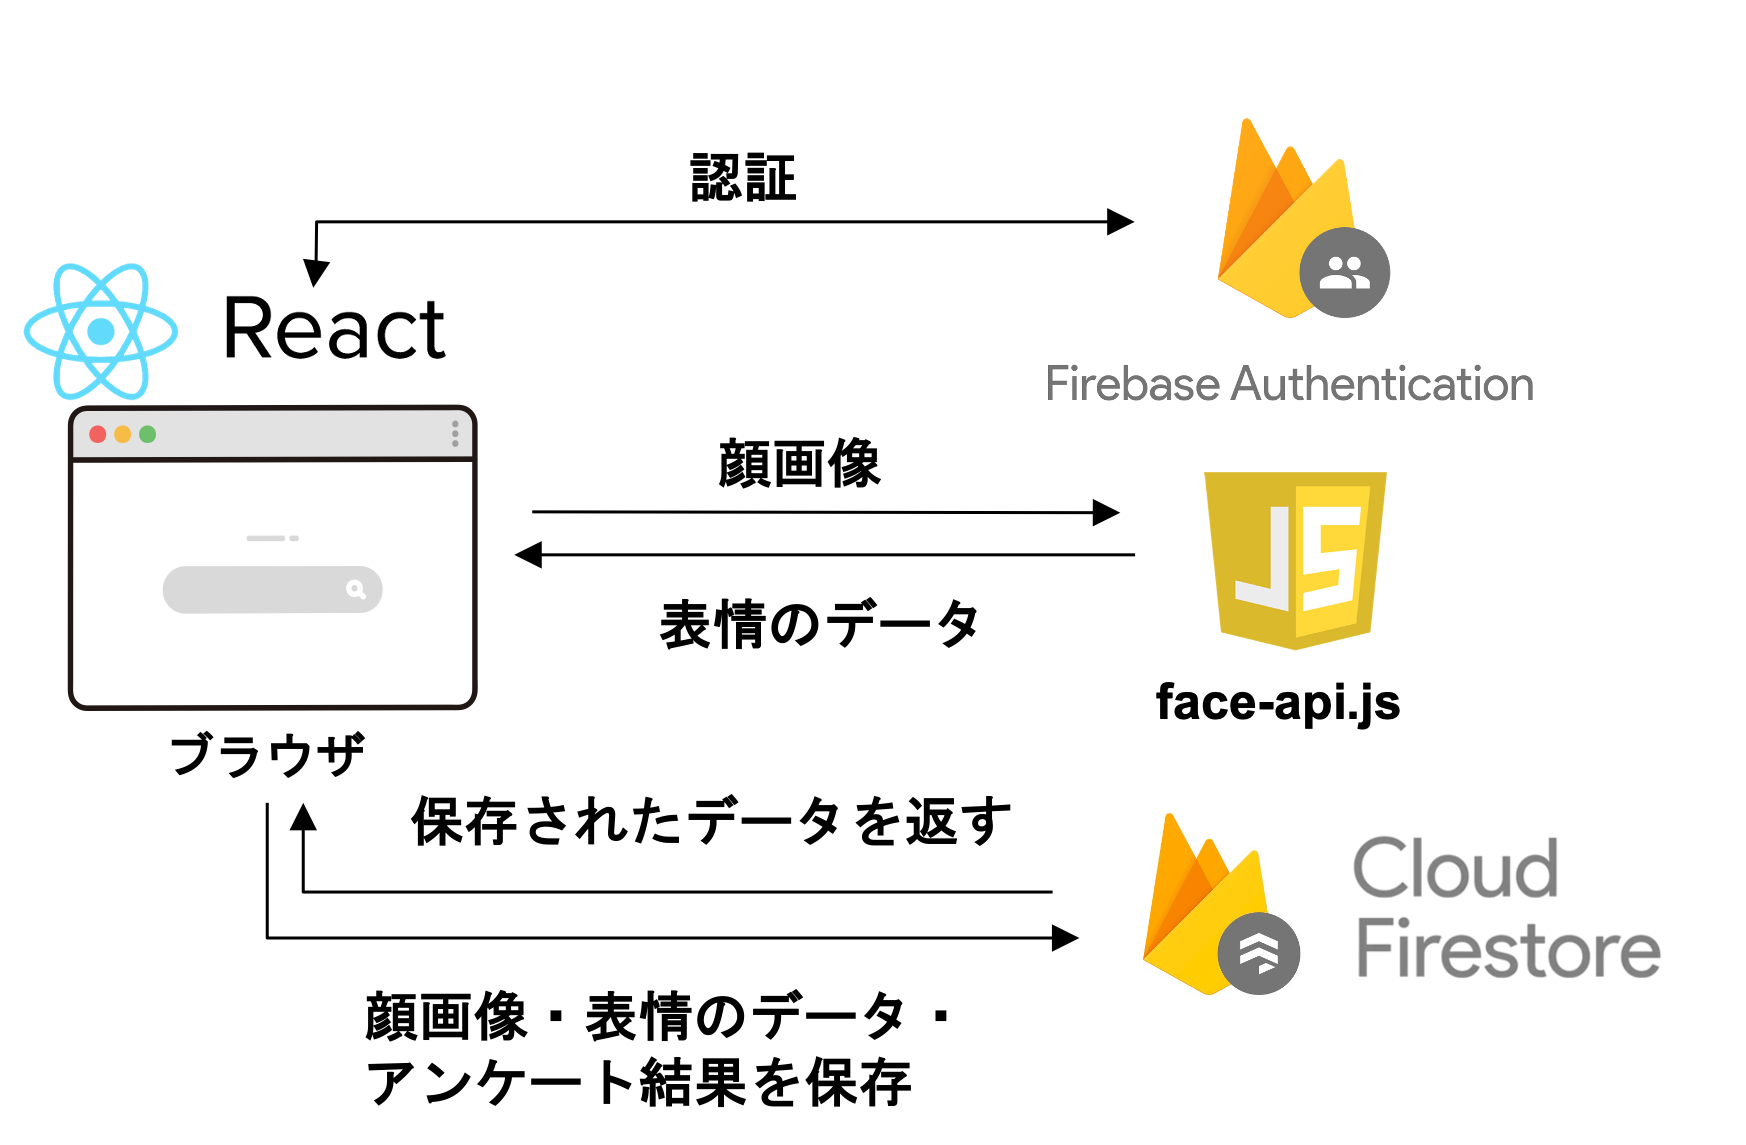
\includegraphics[scale=1.2, clip]{./img/compose.png}
			\caption{システム構成図}
			\label{fig:図の名前}
	\end{center}
\end{figure}


\section{Reactについて}
\label{sec:reference_quote}
Reactは,UI(ユーザインタフェース)部分の構築に特化したJavaScriptのライブラリで,
React.jsとも呼ばれる.
SNSで有名なMeta社(旧Facebook社)が自社サービスの機能拡張に伴うコードの複雑化によって
維持管理がしにくくなることを防ぐために開発した.
コーディングコストが少なく,開発規模が大きくなっても管理しやすいといった特長もあり,
現在では開発元であるFacebook社のサービスであるFacebookやInstagramはもちろんのこと,
Yahoo!やAirbnb,Reddit,Netflix,Slack,Uberといった世界的なWebサイトや
Webアプリで利用されるなど,世界中の多くの企業で採用されており,日本でも注目を集める
など,今最も勢いのあるライブラリである.
今回のシステム開発にReactを採用した理由は三つある.

	\begin{enumerate}
		\item パフォーマンスが良い \\
		Reactには,仮想DOM(Virtual Document Object Model)というレンダリング機構が
		備わっている.仮装DOMとは、実際のDOMではなく, React内部に持っている 
		DOMの情報である. Reactを使うと,この仮想DOMと実際のHTML上のDOMを
		比較したときに出てくる違いだけが,毎回HTML上に再適用される.
		そのため画面全体がReactで構成されていたとしても,必要な部分しか更新されず
		非常に高速に動作するため,パフォーマンスが良い.\\

		\item UIコンポーネントのライブラリが多い \\
		Reactは,世界中で使われているため,Reactのライブラリを使ってUIをコンポート化
		するようになってきている.あらかじめButtonやFormなどのUIパーツを
		Reactコンポーネントとして扱えるようにして,セット化したものが多くある.
		これらを使えば,今風の洗練された画面を作ることができる.\\

		\item JavaScriptの知識があれば使える \\
		基本的にReactはJavaScriptで書かれているため,
		JavaScriptの知識があればアプリを開発することができる.
		たとえJavaScriptの開発経験がなくても基本構文を理解していれば開発に
		取り掛かれる.今回,我々はJavaScriptの学習を既に行なっていたので,
		Reactを選んだ.
	\end{enumerate}
	
\section{face-api.jsについて}
\label{sec:reference_bib}
face-api.jsはブラウザ, NodeJSで顔を検出するための,
Tensorflow.jsを活用したJavaScript APIである.
ここでは,face-api.jsがどのような機能を提供しているかを紹介する.
\begin{itemize}
	\item 顔検出 \\
	写真から顔を探して検出する. \\

	\item 顔のランドマーク検出 \\
	検出した顔の目や鼻の位置など,顔の特徴を抽出する上で重要なキーポイントを検出する. \\

	\item 表情認識 \\
	検出した顔の表情を認識する.表情は,「怒り」,「嬉しさ」,「中立」,「恐怖」,「うんざり」,
	「驚き」,「悲しさ」の7種類あり,数値で表される. \\

	\item 年齢推定 \\
	検出した顔の年齢を推定する. \\

	\item 性別認識 \\
	検出した顔の性別を推定する. \\

\end{itemize}
今回は,顔検出と表情認識の機能を使い,表情分析した値をグラフ化することを目的とする.
また,日々の提出された写真の笑顔度に応じてポイントを付け,加算されていく仕組みを作った.
ソースコード3.1にその仕組みを実装したソースコードを示す. \\

\renewcommand{\lstlistingname}{ソースコード}

\begin{lstlisting}[caption=表情分析]
  const handleImage = async () => {
    // 顔を検出して,表情の値を変数detectionに代入する
    const detections = await faceapi
      .detectAllFaces(imgRef.current, new faceapi.TinyFaceDetectorOptions())
      .withFaceExpressions();

    // ここから笑顔度に応じてポイントを付ける

    // happyの値が0.7以上の場合
    if (detections[0].expressions.happy >= 0.7) {
      setObject({
        expressions: {
          angry: detections[0].expressions.angry,
          disgusted: detections[0].expressions.disgusted,
          fearful: detections[0].expressions.fearful,
          happy: detections[0].expressions.happy,
          neutral: detections[0].expressions.neutral,
          sad: detections[0].expressions.sad,
          surprised: detections[0].expressions.surprised,
        },
        // ポイントは3点
        point: 3,
      });
    } else if (
      // happyの値が0.5以上または
      detections[0].expressions.happy >= 0.5 ||
      // surprisedの値が0.7以上または
      detections[0].expressions.surprised >= 0.7 ||
      // neutralの値が0.7以上の場合
      detections[0].expressions.neutral >= 0.7
    ) {
      setObject({
        expressions: {
          angry: detections[0].expressions.angry,
          disgusted: detections[0].expressions.disgusted,
          fearful: detections[0].expressions.fearful,
          happy: detections[0].expressions.happy,
          neutral: detections[0].expressions.neutral,
          sad: detections[0].expressions.sad,
          surprised: detections[0].expressions.surprised,
        },
        // ポイントは2点
        point: 2,
      });
    } else if (
      // happyの値が0.3以上または
      detections[0].expressions.happy >= 0.3 ||
      // surprisedの値が0.5以上または
      detections[0].expressions.surprised >= 0.5 ||
      // neutralの値が0.5以上の場合
      detections[0].expressions.neutral >= 0.5
    ) {
      setObject({
        expressions: {
          angry: detections[0].expressions.angry,
          disgusted: detections[0].expressions.disgusted,
          fearful: detections[0].expressions.fearful,
          happy: detections[0].expressions.happy,
          neutral: detections[0].expressions.neutral,
          sad: detections[0].expressions.sad,
          surprised: detections[0].expressions.surprised,
        },
        // ポイントは1点
        point: 1,
      });
    // それ以外場合
    } else {
      setObject({
        expressions: {
          angry: detections[0].expressions.angry,
          disgusted: detections[0].expressions.disgusted,
          fearful: detections[0].expressions.fearful,
          happy: detections[0].expressions.happy,
          neutral: detections[0].expressions.neutral,
          sad: detections[0].expressions.sad,
          surprised: detections[0].expressions.surprised,
        },
        // ポイントは0点
        point: 0,
      });
    }
  };

  // 学習モデルを読み込んでfaceapiを使える様にする
  useEffect(() => {
    const loadModels = () => {
      Promise.all([
        faceapi.nets.tinyFaceDetector.loadFromUri("/models"),
        faceapi.nets.faceLandmark68Net.loadFromUri("/models"),
        faceapi.nets.faceExpressionNet.loadFromUri("/models"),
      ])
        .then(handleImage)
        .catch((e) => console.log(e));
    };

    imgRef.current && loadModels();
  }, []);
\end{lstlisting}
	
\section{Material-UIについて}
\label{sec:reference_material}
Google社が自社のサービスに統一的なデザインを与えるために作成した,
デザインのガイドライン,または仕様書であるMaterial Designを
Reactのコンポーネントとして使えるようにしたものである.
本研究でMaterial Designを取り入れているのは,ユーザーにとってストレスが少なく,
みやすく直感的に操作が出来るといった,使いやすさを目的としているためである.

\section{Firebase Authentication}
\label{sec:reference_auth}
Firebase Authenticationはユーザー認証機能を提供し,ユーザ情報をクラウドで保存してくれる,
Google運営のサービスのことである.認証方法には、主に以下が用意されている.

\begin{itemize}
	\item メールアドレスとパスワードによる認証 \\

	\item 主要なプロバイダーアカウントによる認証 \\
	(Google / Twitter / Facebook / Github / Apple / Yahoo! / Microsoft 等) \\

	\item 匿名認証 \\

	\item カスタム認証 \\

	\item 電話番号認証 \\
\end{itemize}

本システムではFirebase Authenticationのソーシャルログイン機能として
提供されている,Googleサインインを利用してアプリケーションの認証システムを作成した. 
GoogleサインインはユーザーのGoogleアカウントを用いてアプリケーションの
ログインを可能にするシステムである. 
ソースコード3.2にGoogleサインインを実装したソースコードを記載する. \\

\begin{lstlisting}[caption=Googleログインの実装]
  const SignIn = () => {
    // ここからGoogleログイン
  const signInWithGoogle = () => {
    // サインインポップアップ画面を表示
    signInWithPopup(auth, provider).then((result) => {
      // 初めてログインしたかどうかの判定
      const isNewUser = getAdditionalUserInfo(result)?.isNewUser;
      if (isNewUser) {
        addDB();
      } else {
        updateDB();
      }
    });
  };

  // ドキュメント追加
  const addDB = async () => {
    await addDoc(collection(db, "users"), {
      // googleのアカウント名
      name: auth.currentUser.displayName,
      // Gmailアドレス
      email: auth.currentUser.email,
      // ログイン日時
      login: serverTimestamp(),
      // 笑みポイント
      point: 0,
      // 役職
      role: "employee",
      // ユーザーID
      uid: auth.currentUser.uid,
    });
  };

  // ドキュメントフィールド更新
  const updateDB = async () => {
    // ユーザー情報の検索
    const querySnapshot = await getDocs(
      query(collection(db, "users"), where("uid", "==", auth.currentUser.uid))
    );
    // ドキュメントIDの取得
    const docId = querySnapshot.docs.map((doc) => doc.id).toString();
    await updateDoc(doc(db, "users", docId), {
      login: serverTimestamp(),
    });
  };
\end{lstlisting}

\vspace{12mm}

 Firebase Authenticationを使用した理由は,認証の安全性を外部に任せることができるからである.
認証システムは,ユーザーの個人情報を預かることになるため,自前で実装するのは危険であり,
万が一,個人情報が流出してしまうおそれがある.さらに,個人情報を保護して運用していく
リスクとコストもかかってしまう.
そこで外部ライブラリを使用することで,問題点を解決できると考えた. \\
 ソーシャルログイン機能を利用することで,ユーザーは本アプリケーションのIDと
パスワードを覚えておく必要がなくなる.また,IDとパスワードを自分で設定してロ
グインするよりも手順が減るため,ユーザーにログインしてもらうハードルを低くす
ることができる. \\
 

\section{Cloud Firestore}
\label{sec:reference_cloud}
Cloud FirestoreはGoogle社が提供しているモバイルアプリやウェブアプリのためのサーバーレスのNoSQLドキュメント指向データベースである.
リアルタイムでのデータ送受信、柔軟なデータ構造やオフライン時のサポートなどの特徴を持つ.
GCPとFirebaseから提供されており,GCPから提供されているバージョンでは,
前のバージョンであるCloud Databaseとの互換性を持つDatastoreモードとネイティブモードを選択できる.Datastoreモードでは,クライアントライブラリ数やオフラインデータの永続性がないなどのいくつかの機能が制限される. \\
 全てのデータはドキュメント、コレクション、サブコレクションに保存され,
ドキュメントは一意なIDをつけコレクション内に作成される.
そして必要に応じ,ドキュメント内にサブコレクションとして新たなコレクションを追加できる.
表3.1と表3.2では,管理者と社員1対1のチャット機能実装におけるコレクションとサブコレクションのドキュメント構造を示す.
表3.3と3.4では管理者と社員それぞれの基本情報と顔写真の分析結果を格納しているコレクションとサブコレクションのドキュメント構造を示す.
表3.5では掲示板機能で用いているドキュメント構造を示す.

\begin{table}[hbtp]
  \caption{コレクションroomsのドキュメント構造}
  \label{table:data_type}
  \centering
  \begin{tabular}{c|c} \hline
    フィールド名  & データの型   \\ \hline
    admin\_id  & number  \\ 
    admin\_name  & string   \\
    admin\_photoURL  &  string \\
    employee\_id  & number  \\ 
    employee\_name  & string   \\
    employee\_photoURL  &  string \\
    messages  &  subcollection \\ \hline
  \end{tabular}
\end{table}

\begin{table}[hbtp]
  \caption{サブコレクションmessagesのドキュメント構造}
  \label{table:data_type}
  \centering
  \begin{tabular}{c|c} \hline
    フィールド値  & データの型  \\
    createdAt  & timestamp \\
    id  & number  \\
    name  & string  \\
    photoURL  &  string \\
    text  &  string \\ \hline
  \end{tabular}
\end{table}

\begin{table}[hbtp]
  \caption{コレクションusersのドキュメント構造}
  \label{table:data_type}
  \centering
  \begin{tabular}{c|c} \hline
    フィールド名  & データの型   \\ \hline
    email  & string   \\  
    id  & number   \\ 
    login  & timestamp  \\ 
    name  &  string  \\ 
    photoURL  &  string  \\ 
    point  &  number  \\ 
    role  &  string  \\ 
    uid  &  string  \\ 
    expressions  &  subcollection  \\ 
    \hline
  \end{tabular}
\end{table}



\clearpage

\begin{table}[hbtp]
  \caption{サブコレクションexpressionsのドキュメント構造}
  \label{table:data_type}
  \centering
  \begin{tabular}{c|c}\hline
    フィールド値  & データの型 \\\hline 
    date  & string  \\
    id  & number  \\
    angry  & number  \\
    disgusted  &  number  \\
    neutral  &  number  \\
    sad  &  number  \\
    fearful  &  number  \\
    surprised  &  number  \\
    happy  &  number  \\\hline
  \end{tabular}
\end{table}

\begin{table}[hbtp]
  \caption{postsのデータ構造}
  \label{table:data_type}
  \centering
  \begin{tabular}{c|c} \hline
    データの型  & 宣言   \\ \hline 
    name  & string  \\
    photoURL  & string  \\
    text  &  string \\ \hline
  \end{tabular}
\end{table}
